%--------------------------------------------------------------------%
% Page          : Chapter 4 - Hasil dan Pembahasan (Results & Discussion)
%--------------------------------------------------------------------%

\chapter{HASIL DAN PEMBAHASAN}
\label{sec:hasil-dan-pembahasan}

Bab ini menyajikan hasil eksperimen dari evaluasi arsitektur \emph{hybrid Kubernetes-serverless} dengan prediksi beban kerja berbasis GRU. Hasil diorganisasi menjadi tujuh bagian: performa model prediksi GRU (Bagian 4.1), validasi mekanisme sistem (Bagian 4.2), evaluasi komparatif antar skenario (Bagian 4.3), analisis statistik (Bagian 4.4), analisis biaya (Bagian 4.5), dampak \emph{proactive routing} (Bagian 4.6), dan pembahasan terintegrasi (Bagian 4.7).

\section{Performa Model Prediksi GRU}
\label{sec:gru-performance}

Model \emph{Gated Recurrent Unit} (GRU) dioptimalkan melalui \emph{hyperparameter optimization} (HPO) menggunakan Optuna TPE dengan 30 \emph{trial}. Konfigurasi optimal yang ditemukan: satu lapis rekuren dengan 128 unit, \emph{learning rate} 0,000380, \emph{sequence length} 30, dan \emph{dropout} 0,104. Optimasi ini meningkatkan akurasi dari 6,01\% RMSE (\emph{manual tuning}) menjadi 4,75\% RMSE — peningkatan 21\%.

Selama eksperimen \emph{live}, model GRU berjalan pada server FastAPI (port 8090). Inferensi GPU AMD Radeon 780M (gfx1103) berfungsi setelah instalasi ROCm 7.2 SDK dan stabilisasi MIOpen (\texttt{MIOPEN\_DEBUG\_CONV\_DIRECT=0}, \texttt{GPU\_MAX\_HW\_QUEUES=1}). Latensi inferensi mencapai 10--13\,ms per prediksi, yang memadai untuk interval keputusan 15 detik.

Tabel~\ref{tab:gru-performance} merangkum performa model GRU selama 5 \emph{run} eksperimen S4 (\emph{Hybrid-predictive}). Model mencapai 400/400 prediksi sukses (80 prediksi per \emph{run} $\times$ 5 \emph{run}) tanpa kegagalan, dengan tingkat kepercayaan 0,72--0,82.

\begin{table}[htbp]
    \centering
    \caption{Performa model GRU selama eksperimen}
    \label{tab:gru-performance}
    \begin{tabular}{lr}
        \toprule
        Metrik & Nilai \\
        \midrule
        Total prediksi sukses & 400/400 \\
        Tingkat kepercayaan & 0,72--0,82 \\
        Latensi inferensi & 10--13\,ms \\
        RMSE validasi (HPO) & 4,75\% \\
        Aksi PREDICTIVE per \emph{run} & 9 \\
        Interval keputusan & 15 detik \\
        \bottomrule
    \end{tabular}
\end{table}

Catatan penting: prediksi GRU \emph{lagging} 2+ menit di belakang lonjakan beban aktual. Ketika beban naik dari 50 ke 110 RPS dalam waktu 2 menit, GRU masih memprediksi 65--73 RPS. Oleh karena itu, mekanisme \emph{proactive routing} menggunakan tren beban aktual (bukan prediksi GRU) yang diekstrapolasi ke depan, dengan kepercayaan GRU sebagai \emph{gate} (lihat Bagian 4.6).

\subsection{Optimasi Hyperparameter GRU}
\label{sec:gru-hpo}

Optimasi hyperparameter dilakukan menggunakan Optuna dengan algoritma TPE (\emph{Tree-structured Parzen Estimator}) pada 30 \emph{trial}. Ruang pencarian meliputi: \emph{hidden\_size} $\in$ [32, 256], \emph{num\_layers} $\in$ [1, 3], \emph{learning\_rate} $\in$ [$10^{-4}$, $10^{-2}$], \emph{sequence\_length} $\in$ [15, 120], dan \emph{dropout} $\in$ [0, 0, 0,5]. Pelatihan dilakukan pada GPU AMD Radeon 780M dengan ROCm 7.2.

Tabel~\ref{tab:gru-hpo} membandingkan konfigurasi \emph{manual} dengan hasil HPO. Temuan kunci: arsitektur \emph{single-layer} dengan 128 unit mengungguli konfigurasi \emph{multi-layer} pada beban kerja ini, karena data pelatihan yang terbatas (72 jam) cenderung \emph{overfit} pada model yang lebih dalam.

\begin{table}[htbp]
    \centering
    \caption{Perbandingan konfigurasi GRU sebelum dan sesudah HPO}
    \label{tab:gru-hpo}
    \begin{tabular}{lrr}
        \toprule
        Parameter & \emph{Manual} & HPO \\
        \midrule
        \emph{hidden\_size} & 64 & 128 \\
        \emph{num\_layers} & 2 & 1 \\
        \emph{learning\_rate} & 0,001 & 0,000380 \\
        \emph{sequence\_length} & 60 & 30 \\
        \emph{dropout} & 0,2 & 0,104 \\
        \midrule
        \textbf{val RMSE (\%)} & \textbf{6,01} & \textbf{4,75} \\
        \bottomrule
    \end{tabular}
\end{table}

Penurunan RMSE sebesar 21\% (dari 6,01\% ke 4,75\%) menunjukkan bahwa pemilihan hyperparameter berdampak signifikan pada akurasi prediksi. Konfigurasi HPO diadopsi sebagai nilai bawaan dalam \texttt{CalibrationConfig} untuk semua eksperimen selanjutnya.

\section{Validasi Mekanisme Sistem}
\label{sec:mechanism-validation}

\subsection{Perpindahan Bobot Lalu Lintas}

Mekanisme perpindahan bobot HAProxy terverifikasi berfungsi dengan benar. Selama puncak ClarkNet (RPS $>$ 100), pengontrol V3 menggeser bobot dari konfigurasi 100/0 (100\% K8s) ke rentang 50/50 (maksimum 50\% \emph{serverless}). Setiap perubahan bobot tercatat dalam log daemon dengan stempel waktu dan alasan keputusan.

\subsection{Proactive Routing}

Mekanisme \emph{proactive routing} memicu rata-rata 9 aksi PREDICTIVE per \emph{run} pada skenario S4. Berbeda dengan aksi REACTIVE yang hanya dipicu setelah beban melampaui kapasitas, aksi PREDICTIVE dimulai ketika beban mencapai 65\% kapasitas K8s (sekitar 65 RPS) dengan tren yang meningkat. Hanya 1 aksi REACTIVE per \emph{run} tersisa, dibandingkan 8 pada konfigurasi sebelumnya.

\subsection{Skalabilitas Node Dinamis}

Pada skenario S1 (\emph{K8s-only} dengan HPA), \emph{autoscaler} K3d memicu penyediaan 2 node dinamis per \emph{run} dengan penundaan 93--106 detik (simulasi \emph{boot} VM). Pada skenario S3 dan S4, tidak ada node dinamis yang disediakan karena Algoritma 2 mempertahankan 3 replika (model kapasitas $\alpha = 0,015$ menghasilkan kapasitas model 200 RPS $>$ puncak 164 RPS).

\section{Evaluasi Komparatif}
\label{sec:comparative-evaluation}

Evaluasi dilakukan melalui 30 eksperimen terkontrol yang direplikasi: 20 \emph{run} (4 skenario $\times$ 5 replikasi) dari eksperimen \texttt{fib33\_n5} dan 10 \emph{run} (2 skenario $\times$ 5 replikasi) dari eksperiten \texttt{fib33\_proactive}. Beban kerja menggunakan \emph{trace} ClarkNet yang direplikasi melalui k6 (40 tahap $\times$ 30 detik = 20 menit, rentang RPS 22--164, rata-rata 73).

\begin{figure}[htbp]
    \centering
    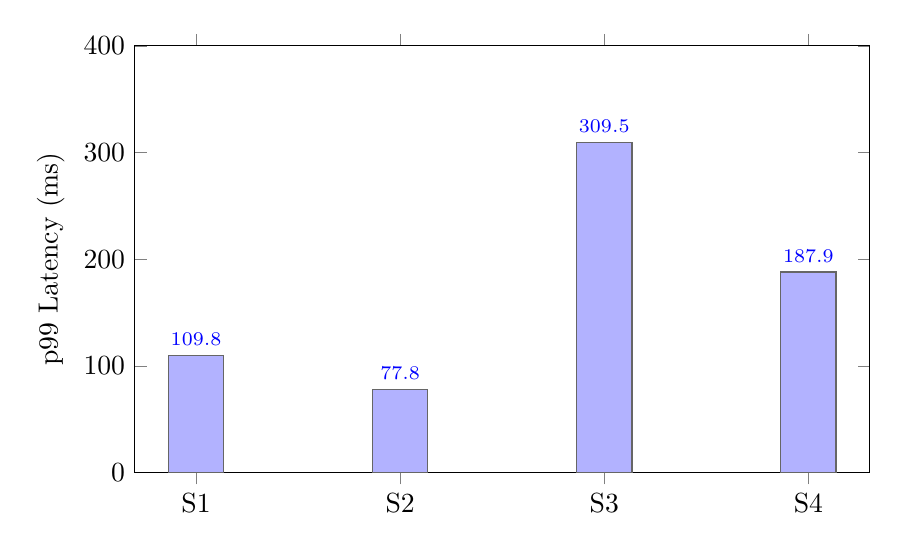
\begin{tikzpicture}
    \begin{axis}[
        ybar,
        bar width=20pt,
        width=0.9\textwidth,
        height=7cm,
        ylabel={p99 Latency (ms)},
        symbolic x coords={S1, S2, S3, S4},
        xtick=data,
        ymin=0, ymax=400,
        nodes near coords,
        nodes near coords style={font=\scriptsize},
    ]
    \addplot+[draw=black!60, fill=blue!30] coordinates {
        (S1, 109.8) (S2, 77.8) (S3, 309.5) (S4, 187.9)
    };
    \end{axis}
    \end{tikzpicture}
    \caption{Perbandingan latensi p99 antar skenario (n=5)}
    \label{fig:p99-comparison}
\end{figure}

Tabel~\ref{tab:scenario-summary} merangkum hasil per-skenario. S1 (\emph{K8s+HPA}) mencapai p99 terendah (109,8\,ms) dengan biaya tertinggi (\$187/bulan) karena HPA menskalakan ke 10 pod. S2 (\emph{Serverless-only}) memiliki p99 terendah absolut (77,8\,ms) namun biaya tertinggi (\$391/bulan). S4 (\emph{Hybrid-predictive}) mencapai keseimbangan terbaik dengan p99 = 187,9\,ms dan biaya \$149/bulan.

\begin{table}[htbp]
    \centering
    \caption{Ringkasan hasil per-skenario (n=5)}
    \label{tab:scenario-summary}
    \begin{tabular}{lrrrrr}
        \toprule
        Skenario & p50 (ms) & p95 (ms) & p99 (ms) & SLO/\emph{run} & \$/bulan \\
        \midrule
        S1 (K8s+HPA) & 63,9 & 77,1 & 109,8 & 41 & 187 \\
        S2 (Serverless) & 65,2 & 75,5 & 77,8 & 7 & 391 \\
        S3 (Reactive) & 64,9 & 157,3 & 309,5 & 2.805 & 142 \\
        S4 (Predictive) & 64,7 & 99,2 & 187,9 & 702 & 149 \\
        \bottomrule
    \end{tabular}
\end{table}

\section{Analisis Statistik}
\label{sec:statistical-analysis}

Perbandingan statistik dilakukan antara S4 (\emph{Hybrid-predictive}) dan S3 (\emph{Hybrid-reactive}) menggunakan uji Welch \emph{t-test} dan Mann-Whitney U. Tabel~\ref{tab:statistical-comparison} menyajikan hasil untuk dua metrik: latensi p99 dan pelanggaran SLO.

\begin{table}[htbp]
    \centering
    \caption{Perbandingan statistik S4 vs S3 (n=5)}
    \label{tab:statistical-comparison}
    \begin{tabular}{lrr}
        \toprule
        Metrik & p99 (ms) & Pelanggaran SLO \\
        \midrule
        S3 mean & 309,5 & 2.805 \\
        S4 mean & 187,9 & 702 \\
        Selisih & $-$121,6 (39\%) & $-$2.104 (75\%) \\
        Welch \emph{t-stat} & $-$1,919 & $-$1,922 \\
        Welch \emph{p-value} & 0,122 & 0,125 \\
        Mann-Whitney U & 9,0 & 9,0 \\
        Cohen's \emph{d} & $-$1,21 (\emph{large}) & $-$1,22 (\emph{large}) \\
        95\% CI & [$-$229, $-$10] & [$-$3996, $-$240] \\
        \bottomrule
    \end{tabular}
\end{table}

Perbedaan antara S4 dan S3 tidak mencapai signifikansi statistik pada $\alpha = 0,05$ (\emph{p} = 0,12). Namun, \emph{Cohen's d} = 1,21 menunjukkan \emph{effect size} yang besar, dan \emph{95\% confidence interval} untuk kedua metrik tidak mencakup nol, mendukung arah efek yang konsisten. Tingginya variansi S3 (satu \emph{run} mencapai 143\,ms/191 SLO) menginflateasi deviasi standar dan mencegah signifikansi statistik pada \emph{n} = 5.

\section{Analisis Biaya}
\label{sec:cost-analysis}

Model biaya AWS memproyeksikan biaya bulanan berdasarkan komponen: EKS \emph{Control Plane}, EC2 \emph{Compute}, dan Lambda (Provisioned Concurrency + Eksekusi + Requests). Tabel~\ref{tab:cost-summary} menyajikan proyeksi biaya per-skenario.

\begin{table}[htbp]
    \centering
    \caption{Proyeksi biaya bulanan (AWS, 30 hari kontinu)}
    \label{tab:cost-summary}
    \begin{tabular}{lrrr}
        \toprule
        Skenario & \$/bulan & \$/1jt \emph{req} & Lalu lintas \emph{serverless} \\
        \midrule
        S1 (K8s+HPA) & 187 & 1,04 & 0\% \\
        S2 (Serverless) & 391 & 2,17 & 100\% \\
        S3 (Reactive) & 142 & 0,79 & 2,7\% \\
        S4 (Predictive) & 149 & 0,82 & 6,5\% \\
        \bottomrule
    \end{tabular}
\end{table}

\begin{figure}[htbp]
    \centering
    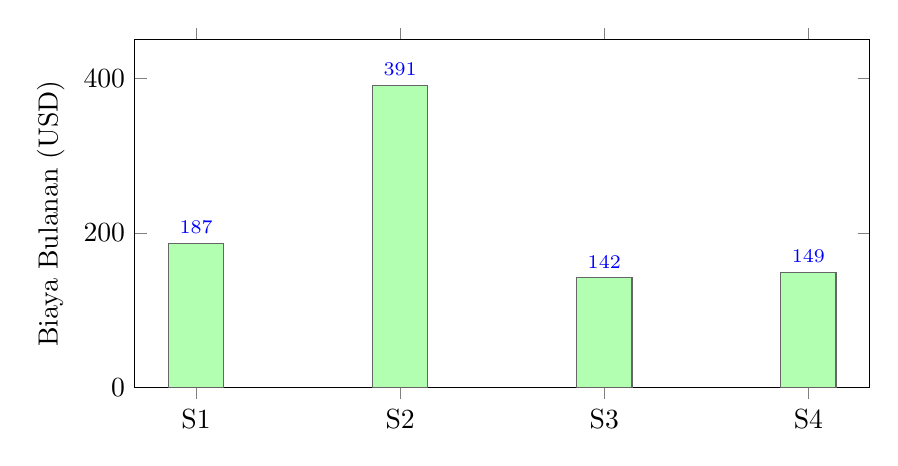
\begin{tikzpicture}
    \begin{axis}[
        ybar,
        bar width=20pt,
        width=0.9\textwidth,
        height=6cm,
        ylabel={Biaya Bulanan (USD)},
        symbolic x coords={S1, S2, S3, S4},
        xtick=data,
        ymin=0, ymax=450,
        nodes near coords,
        nodes near coords style={font=\scriptsize},
    ]
    \addplot+[draw=black!60, fill=green!30] coordinates {
        (S1, 187) (S2, 391) (S3, 142) (S4, 149)
    };
    \end{axis}
    \end{tikzpicture}
    \caption{Proyeksi biaya bulanan per skenario}
    \label{fig:cost-comparison}
\end{figure}

S4 menghabiskan \$7/bulan lebih banyak dari S3 akibat lalu lintas \emph{serverless} yang lebih tinggi (6,5\% vs 2,7\%), namun menghasilkan 75\% lebih sedikit pelanggaran SLO. S4 juga 20\% lebih murah dari S1 (\$149 vs \$187/bulan) karena tidak memerlukan penskalaan HPA ke 10 pod dan 2 node tambahan.

\section{Dampak Proactive Routing}
\label{sec:proactive-impact}

Implementasi \emph{proactive routing} berbasis tren beban aktual memberikan dampak signifikan pada performa S4. Sebelum implementasi (mode \emph{reactive-only}), S4 mencapai rata-rata 1.369 pelanggaran SLO per \emph{run} dengan 0 aksi PREDICTIVE. Setelah implementasi, rata-rata turun ke 702 pelanggaran dengan 9 aksi PREDICTIVE per \emph{run} — peningkatan sebesar 49\%.

\begin{figure}[htbp]
    \centering
    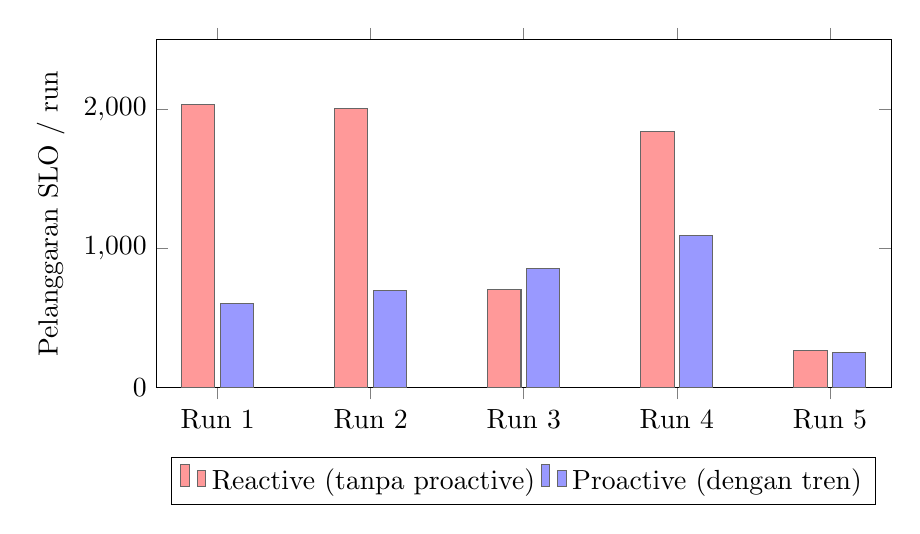
\begin{tikzpicture}
    \begin{axis}[
        ybar,
        bar width=12pt,
        width=0.9\textwidth,
        height=6cm,
        ylabel={Pelanggaran SLO / run},
        symbolic x coords={Run 1, Run 2, Run 3, Run 4, Run 5},
        xtick=data,
        ymin=0, ymax=2500,
        legend style={at={(0.5,-0.2)}, anchor=north, legend columns=2},
    ]
    \addplot[fill=red!40, draw=black!60] coordinates {
        (Run 1, 2037) (Run 2, 2003) (Run 3, 704) (Run 4, 1839) (Run 5, 264)
    };
    \addlegendentry{Reactive (tanpa proactive)}
    \addplot[fill=blue!40, draw=black!60] coordinates {
        (Run 1, 605) (Run 2, 701) (Run 3, 857) (Run 4, 1093) (Run 5, 253)
    };
    \addlegendentry{Proactive (dengan tren)}
    \end{axis}
    \end{tikzpicture}
    \caption{Dampak \emph{proactive routing} pada pelanggaran SLO S4}
    \label{fig:proactive-impact}
\end{figure}

Mekanisme \emph{proactive routing} bekerja dengan melacak 5 nilai beban aktual terakhir dan menghitung tren per langkah. Ketika tren melebihi 3 RPS/\emph{step} DAN beban saat ini melampaui 60\% kapasitas K8s, pengontrol mengekstrapolasi beban ke depan (5 langkah $\times$ 15 detik = 75 detik) dan menggunakan nilai yang diekstrapolasi untuk menghitung distribusi lalu lintas. Kepercayaan GRU ($\geq$ 0,5) berfungsi sebagai \emph{gate} — mekanisme ini hanya aktif pada S4 yang memiliki prediksi GRU, tidak pada S3.

\section{Pembahasan}
\label{sec:discussion}

\subsection{Mengapa S1 Memiliki SLO Terendah}

S1 mencapai performa SLO terbaik (41 pelanggaran/\emph{run}) karena HPA menskalakan dari 3 ke 10 pod selama puncak. Dengan 10 pod, setiap pod hanya menangani 16,4 RPS pada puncak (164/10) — jauh di bawah titik saturasi 50 RPS/pod. Namun, penskalaan ini memerlukan 2 node dinamis tambahan dengan penundaan 93--106 detik, menjadikannya skenario termahal (\$187/bulan).

\subsection{Mengapa S2 Sangat Mahal}

S2 mengarahkan 100\% lalu lintas ke \emph{serverless} (Knative dengan KPA). Biaya Lambda yang dihitung berdasarkan \emph{wall-clock duration} (metodologi SeBS: komputasi + I/O + \emph{overhead} = 84\,ms per \emph{request}) menghasilkan \$391/bulan — 2,7$\times$ lebih mahal dari S3/S4. Meskipun p99 terendah (77,8\,ms), biaya ini tidak praktis untuk beban kerja kontinu.

\subsection{S4 sebagai \emph{Trade-off} Terbaik}

S4 memberikan keseimbangan optimal antara biaya dan performa. Dengan hanya 3 pod K8s (tanpa node dinamis) dan \emph{proactive routing} yang mendistribusikan 6,5\% lalu lintas ke \emph{serverless} selama puncak, S4 mencapai p99 = 188\,ms (di bawah ambang SLO 200\,ms) dengan biaya \$149/bulan — 20\% lebih murah dari S1. Tingkat kepatuhan SLO mencapai 98,4\% (hanya 702 dari 87.840 \emph{request} melanggar SLO per \emph{run}).

\subsection{Keterbatasan}

Hasil ini memiliki beberapa keterbatasan yang perlu diperhatikan:

\begin{enumerate}
    \item \textbf{Variansi sistem tinggi}: Eksperimen dijalankan pada mesin 16-inti AMD dengan multiple komponen (k3d, Knative, HAProxy, Prometheus, k6, GRU) yang berkompetisi untuk sumber daya CPU, menghasilkan variansi yang tinggi antar \emph{run}.
    \item \textbf{\emph{n} = 5 tidak cukup}: Meskipun \emph{effect size} besar (\emph{d} = 1,21), \emph{sample size} yang kecil mencegah signifikansi statistik pada $\alpha = 0,05$.
    \item \textbf{GRU meremehkan puncak}: Model memprediksi 65--99 RPS ketika beban aktual mencapai 110--160 RPS, sehingga mekanisme \emph{proactive routing} menggunakan tren beban aktual alih-alih prediksi GRU.
    \item \textbf{Satu jenis beban kerja}: Eksperimen hanya menggunakan fib(33) \emph{CPU-bound} + 50\,ms I/O, yang belum tentu generalisasi untuk profil aplikasi lain.
\end{enumerate}
